\chapter{Metodología} \label{sec:Metodos}

%Describe la metodología para la medición de calidad de energía

\section{Sistema eléctrico, S/E 191, 192, 193 y 194}

%Describe el sistema eléctrico donde se realizo la medición (Imágenes de diagramas unifilares)

\section{Procedimiento de medición}

%Describe el procedimiento y los requerimientos como son facturas, inspección visual y demás para realizar la medición.

\section{Equipo}

%Recuerda describir mas las características del equipo, coloca imágenes del equipo y sus conexiones, imágenes de la aplicación y demás.

Las mediciones se realzaron con un equipo analizador de red eléctrica con las siguientes características:

\begin{table}[H]
%\small
%\footnotesize
%\scriptsize
%\tiny
\begin{center}
\begin{tabular}{| c | c | c |}
 \hline
    \textbf{MARCA}    & \textbf{MODELO} & \textbf{PERIODO DE MEDICIÓN} \\  
 \hline
      CIRCUITOR       &   MYeBOX 1500   &        1 minuto              \\
 \hline
\end{tabular}
\caption{Características del equipo analizador de red eléctrica utilizado.}
\label{Table:Caract_MYeBOX}
\end{center}
\end{table}

Se realiza la instalación del equipo para medir las siguientes variables en la red eléctrica:

\begin{itemize}
    \item \textbf{Parámetros eléctricos:} Tensión, corriente, frecuencia.
    \item \textbf{Potencia y energía:} Activa, reactiva, aparente, factor de potencia.
    \item \textbf{Armónicos:} Distorsión armónica total en tensión (THD) y en corriente (TDD).
\end{itemize} 

\section{Puntos de medición}

Se realiza medición sobre la Subestación 191, 192, 193 y 194 en la ciudad de Cartagena.


\begin{figure}[H]
\centering
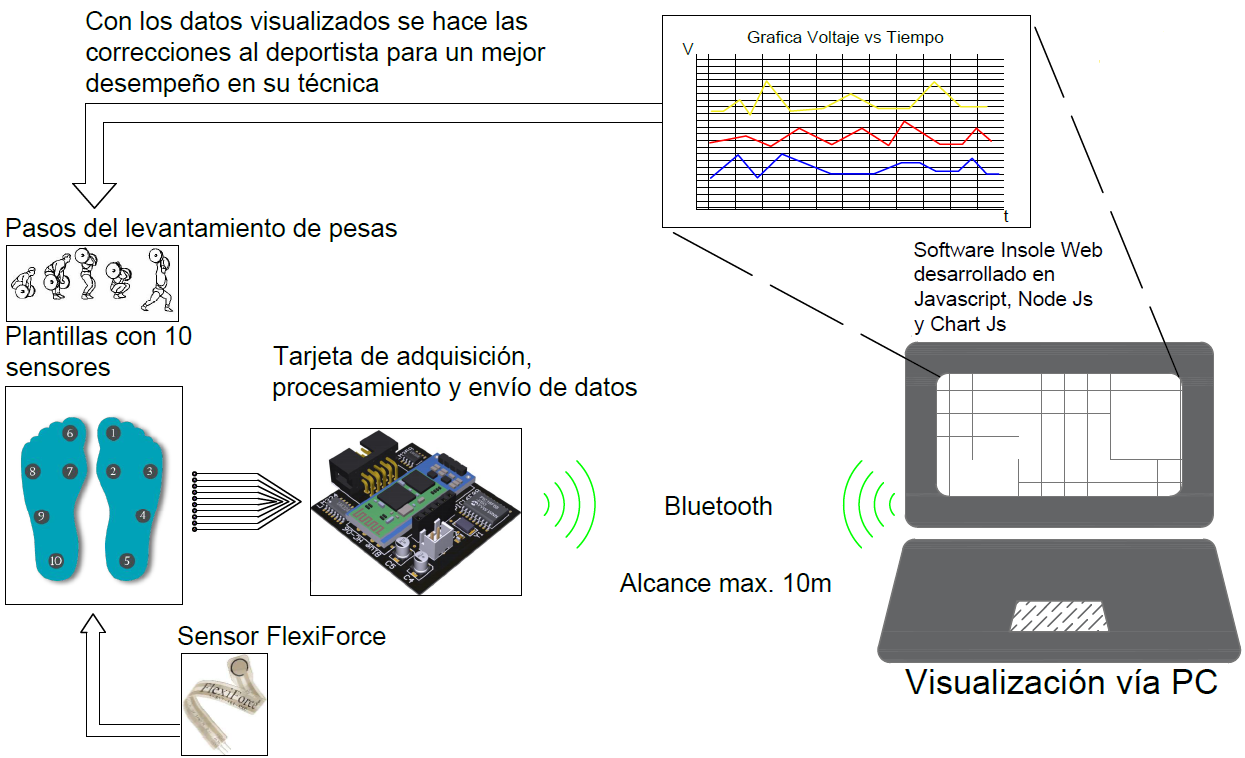
\includegraphics[width=0.83\textwidth]{./image/Diagrama_de_Bloques_sistema_Insole.png}
\caption{Diagrama de Bloques del sistema de adquisición de datos.}
\label{fig:DiagramaBloque}
\end{figure}


\section{Evaluación del Sensor}

\begin{wrapfigure}{r}{0.3\linewidth}
\centering
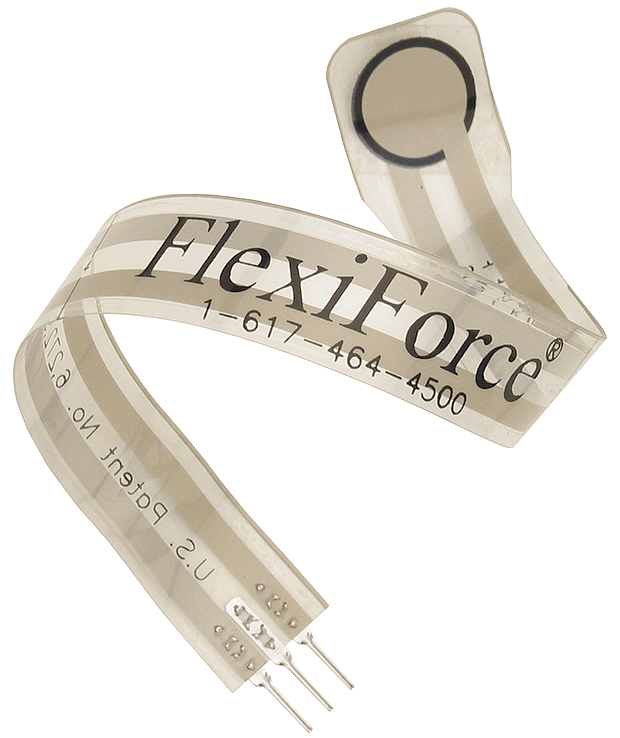
\includegraphics[width=0.2\textwidth]{./image/SensorFlexiForce.png}
\caption{Sensor FlexiForce 100 lbs Tekscan, Piezorresistivo.}
\label{fig:Sensor}
\end{wrapfigure}

El sensor utilizado es el Flexiforce A201, un sensor piezoresistivo delgado y flexible. A mayor fuerza ejercida, la resistencia del sensor se reduce. Las dimensiones del sensor no cambian cuando se flexiona, su rango de fuerza es de $(0-100lbs)$ $440N$, temperatura limite es de $(-9^\circ C$ hasta $60^\circ C)$ y el tiempo de respuesta es de $5$ microsegundos. Con las especificaciones técnicas de los sensores, se diseñaron los circuitos electrónicos para la adquisición de las señales, conversión A/D, y procesamiento.

\begin{figure}[H]
\centering
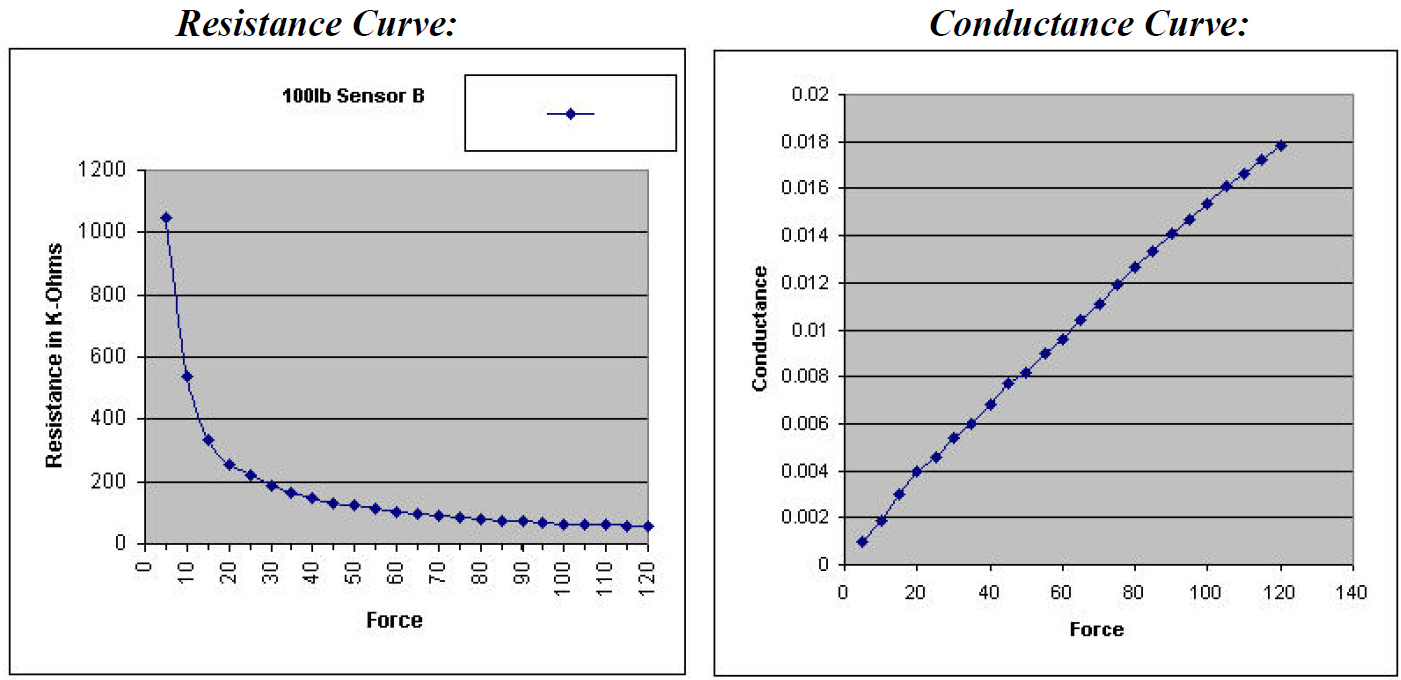
\includegraphics[width=0.9\textwidth]{./image/Curve.png}
\caption{Curvas de Calibración. Fuente: {\href{https://smartxpwiki.ewi.utwente.nl/_media/flx-flexiforce-sensors-manual.pdf}{FlexiForce Sensors Manual.}}}
\label{fig:Curvas}
\end{figure}

\section{Microcontrolador PIC16F88}
Para la selección del microcontrolador se tuvieron en cuenta los siguientes aspectos: el número de pines de entrada analógicos, la opción de empaquetado de montaje superficial y que trabajara con puertos series como son Rx y Tx a 9600 baudios para un correcto funcionamiento con el Bluetooth. Teniendo en cuenta las características anteriormente mencionadas, se eligió el \href{http://ww1.microchip.com/downloads/en/DeviceDoc/30487c.pdf}{PIC16F88} de \href{http://www.microchip.com/}{Microchip} y sus características son presentadas a continuación:

\textbf{Características de baja potencia:}
\begin{itemize}
\item Modos de administración de potencia:
	\begin{itemize}
	\item Primary Run: RC oscillator, 76 $\mu$A, 1MHz, 2V
    \item RC\_RUN: 7 $\mu$A, 31.25kHz, 2V
    \item SEC\_RUN: 9 $\mu$A, 32 kHz, 2V
    \item Sleep: 0.1 $\mu$A, 2V
	\end{itemize}
\item Timer1 Oscillator: 1.8 $\mu$A, 32 kHz, 2V
\item Watchdog Timer: 2.2 $\mu$A, 2V
\item Two-Speed Oscillator Start-up
\end{itemize}

\textbf{Características de los periféricos:}
\begin{itemize}
\item Capture, Compare, PWM (CCP) module:
	\begin{itemize}
	\item Capture is 16-bit, max. resolution is 12.5 ns
    \item Compare is 16-bit, max. resolution is 200 ns
    \item PWM max. resolution is 10-bit
	\end{itemize}
\item 10-bit, 7-channel Analog-to-Digital Converter
\item Synchronous Serial Port (SSP) with SPI™ (Master/Slave) and I$^{2}$C™ (Slave)
\item Addressable Universal Synchronous Asynchronous Receiver Transmitter (AUSART/SCI) with 9-bit address detection:
	\begin{itemize}
	\item RS-232 operation using internal oscillator (no external crystal required)
	\end{itemize}
\item Dual Analog Comparator module:
	\begin{itemize}
	\item Programmable on-chip voltage reference
    \item Programmable input multiplexing from device inputs and internal voltage reference
    \item Comparator outputs are externally accessible
	\end{itemize}
\end{itemize}

\textbf{Características especiales del Microcontrolador:}
\begin{itemize}
\item 100.000 erase/write cycles Enhanced Flash program memory typical
\item 1.000.000 typical erase/write cycles EEPROM data memory typical
\item EEPROM Data Retention: > 40 years
\item In-Circuit Serial Programming™ (ICSP™) via two pins
\item Processor read/write access to program memory
\item Low-Voltage Programming
\item In-Circuit Debugging via two pins
\item Extended Watchdog Timer (WDT):
	\begin{itemize}
	\item Programmable period from 1 ms to 268s
	\end{itemize}
\item Wide operating voltage range: 2.0V to 5.5V
\end{itemize}

\begin{figure}[H]
\centering
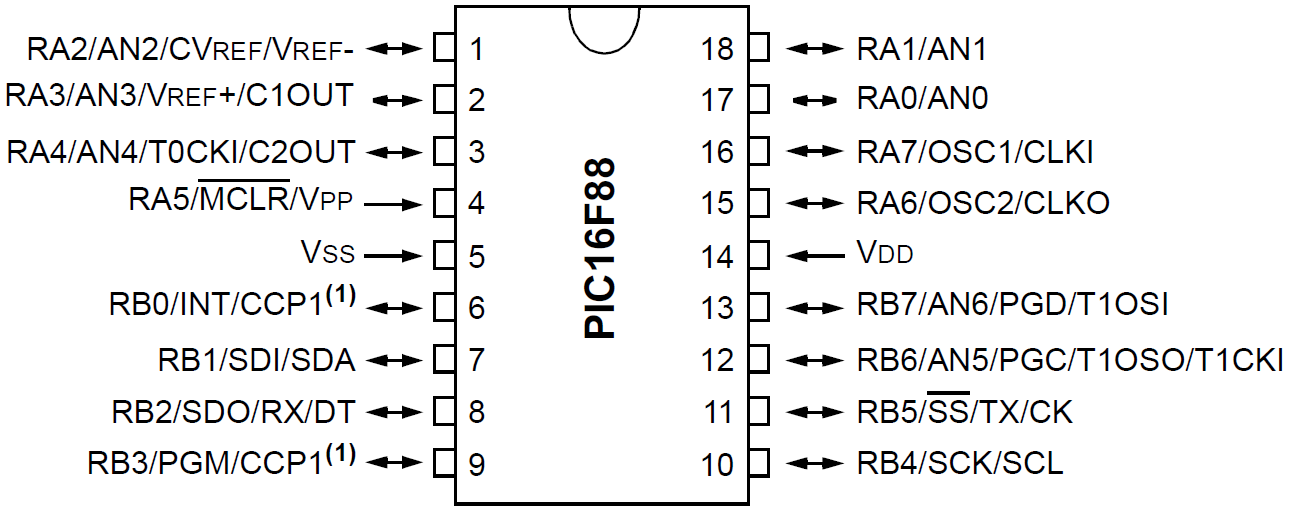
\includegraphics[width=0.9\textwidth]{./image/PIC16F88.png}
\caption{Diagrama de pines PIC16F88.}
\label{fig:PIC16F88}
\end{figure}


\section{Modulo Bluetooth HC-06}

Se seleccionó la tecnología Bluetooth por su bajo consumo de potencia, alcance y bajo costo. Las características del modulo HC-06 son:
\begin{itemize}
\item Led indicadores de conexión y encendido.
\item Alcance: 10m aproximados.
\item Compatible con el protocolo Bluetooth V2.0.
\item Voltaje de alimentación: 3.3VDC $\sim$ 6VDC.
\item Voltaje de operación: 3.3VDC.
\item Corriente: < 40 mA
\item Velocidad de comunicación ajustable: 1200, 2400, 4800, 9600, 19200, 38400, 57600, 115200 baud.
\item Medidas: 1.73 in x 0.63 in x 0.28 in (4.4 cm x 1.6 cm x 0.7 cm)
\item Número de pines: 4
\end{itemize}

\begin{figure}[H]
\centering
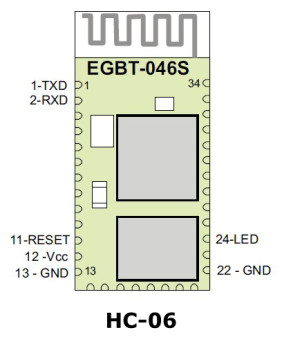
\includegraphics[width=0.3\textwidth]{./image/Blue_HC-06.png}
\caption{Modulo Bluetooth HC-06.}
\label{fig:Blue_HC-06}
\end{figure}

Su reducido tamaño permite cumplir con uno de los objetivos principales de portabilidad del sistema el cual no interviene en la practica del deporte a monitorear. 

\section{Diseño y fabricación del circuito impreso para la adquisición y envío de datos}

Para el diseño del circuito se tienen en cuenta las diferentes etapas que son la alimentación de la tarjeta, la adquisición de datos, el procesamiento de datos y la comunicación para el envío de datos.

\begin{figure}[H]
 \centering
  \subfloat[Software Altium Design versión 18.]{
   \label{fig:AltiumDesign}
    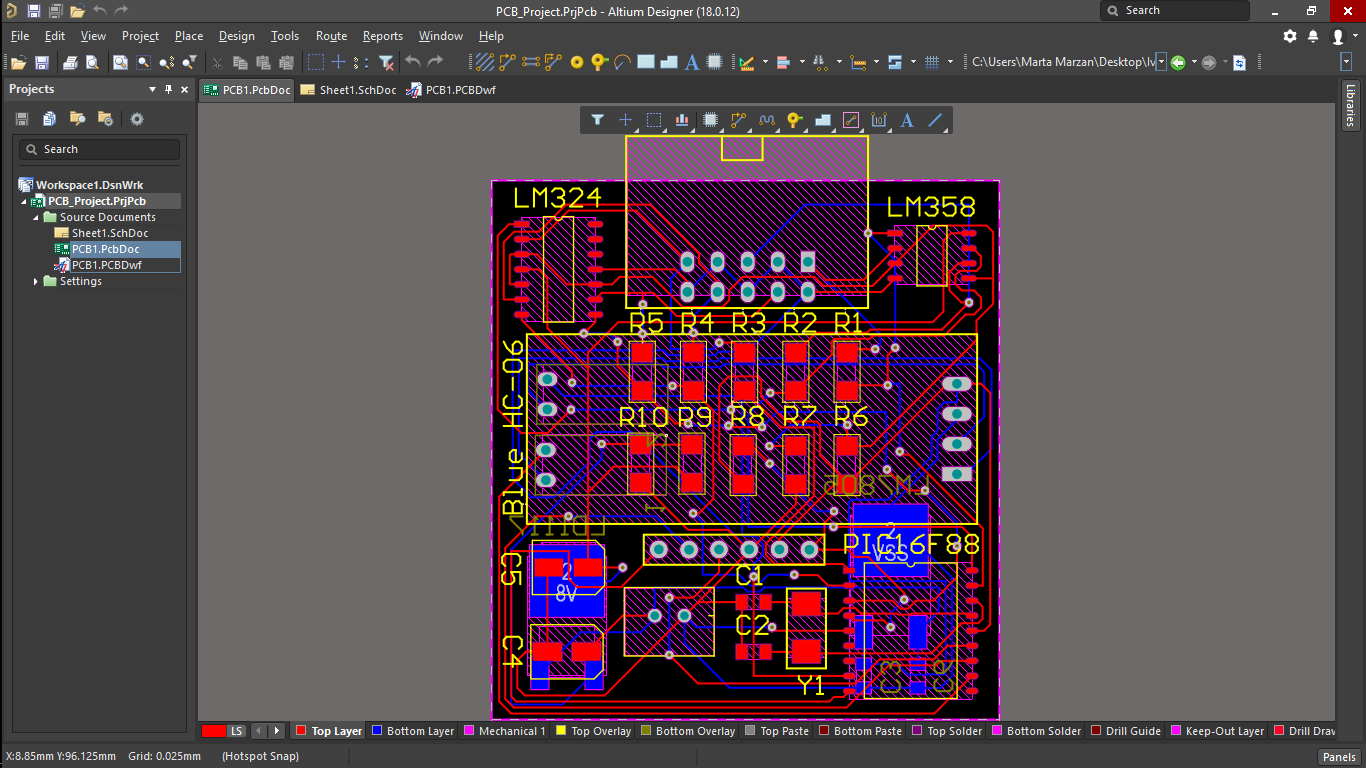
\includegraphics[width=0.49\textwidth]{./image/AltiumDesign.png}}
    \subfloat[Software SolidWorks versión 17.]{
   \label{fig:SolidWorks}
    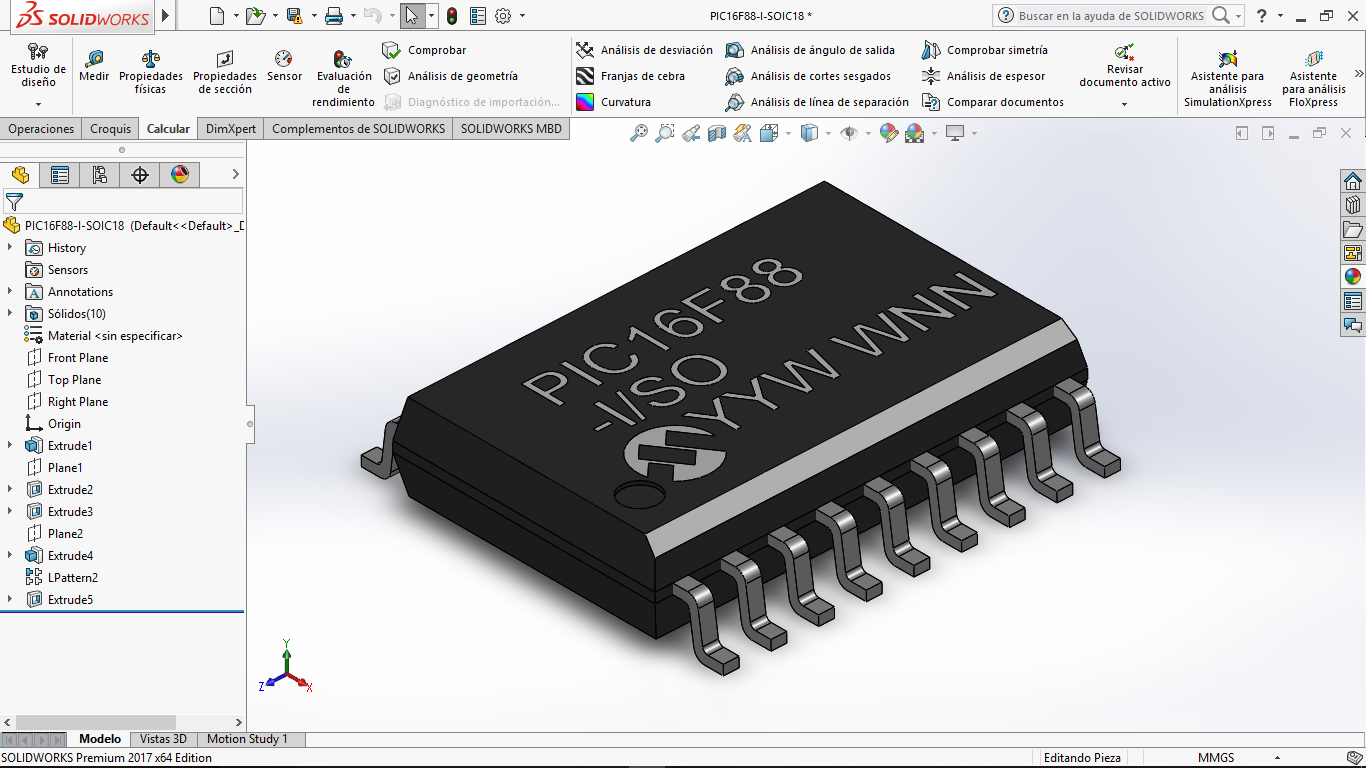
\includegraphics[width=0.49\textwidth]{./image/Solid_PIC16F88_3D.png}}\\
    \subfloat[Software Proteus versión 8.5.]{
   \label{fig:Proteus}
    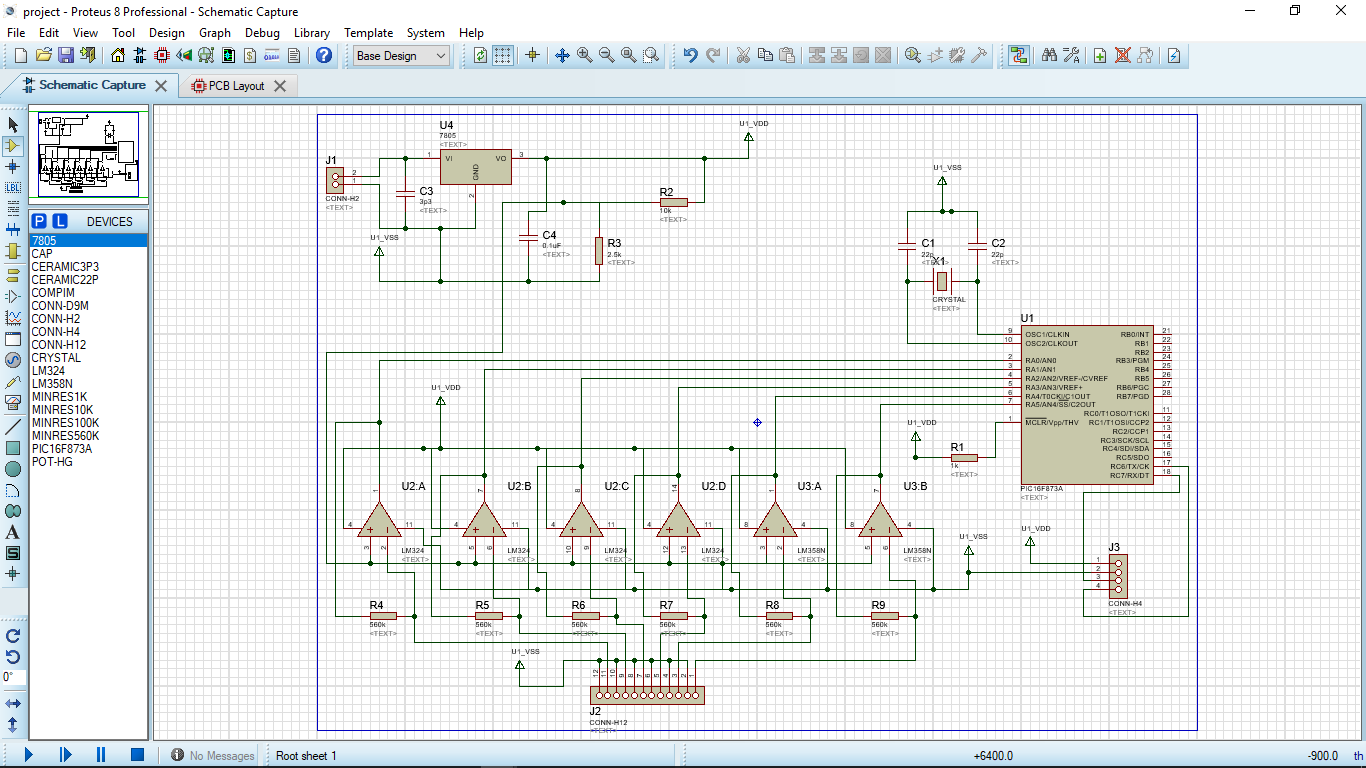
\includegraphics[width=0.49\textwidth]{./image/Proteus_esquematico.png}}
    \subfloat[Software miKroC for PIC versión 17.]{
   \label{fig:mickroC}
    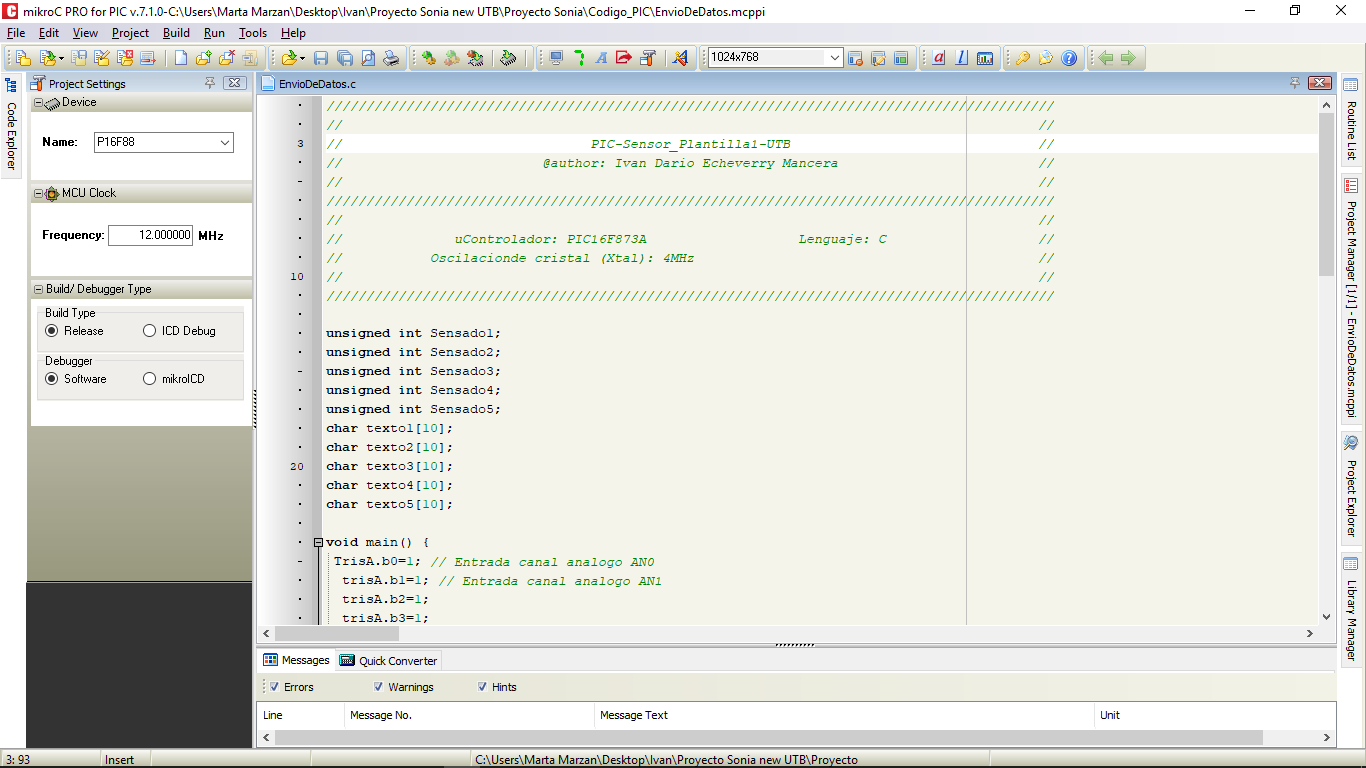
\includegraphics[width=0.49\textwidth]{./image/microC_for_PIC.png}}
 \caption{Tipos de Software utilizados para el diseño del sistema.}
 \label{fig:Software}
\end{figure}

Los programas computacionales utilizados para la simulación, diseño y elaboración de la tarjeta PCB son \href{https://www.labcenter.com/}{Proteus} versión 8.5 de Labcenter y \href{https://www.altium.com/altium-designer/es}{Altium Design} versión 18. Además se utilizó el software de diseño CAD \href{http://www.solidworks.es/}{SolidWorks} versión 17 para el diseño 3D de los componentes del circuito. Este programa se complementa con \href{https://www.altium.com/altium-designer/es}{Altium Design}. Para obtener mejores resultados se utilizaron librerías o modelos ya creados por otros usuarios de SolidWorks que se encuentran alojados en 3DContentCentral (\href{http://www.3dcontentcentral.es/}{http://www.3dcontentcentral.es/}) de forma libre para su desarrollo.

A continuación se describirá el circuito, que consta de las siguientes etapas: etapa (1) de alimentación, etapa (2) de adquisición y acondicionamiento de los datos y etapa (3) de procesamiento y transmisión de datos.

\begin{figure}[H]
\centering
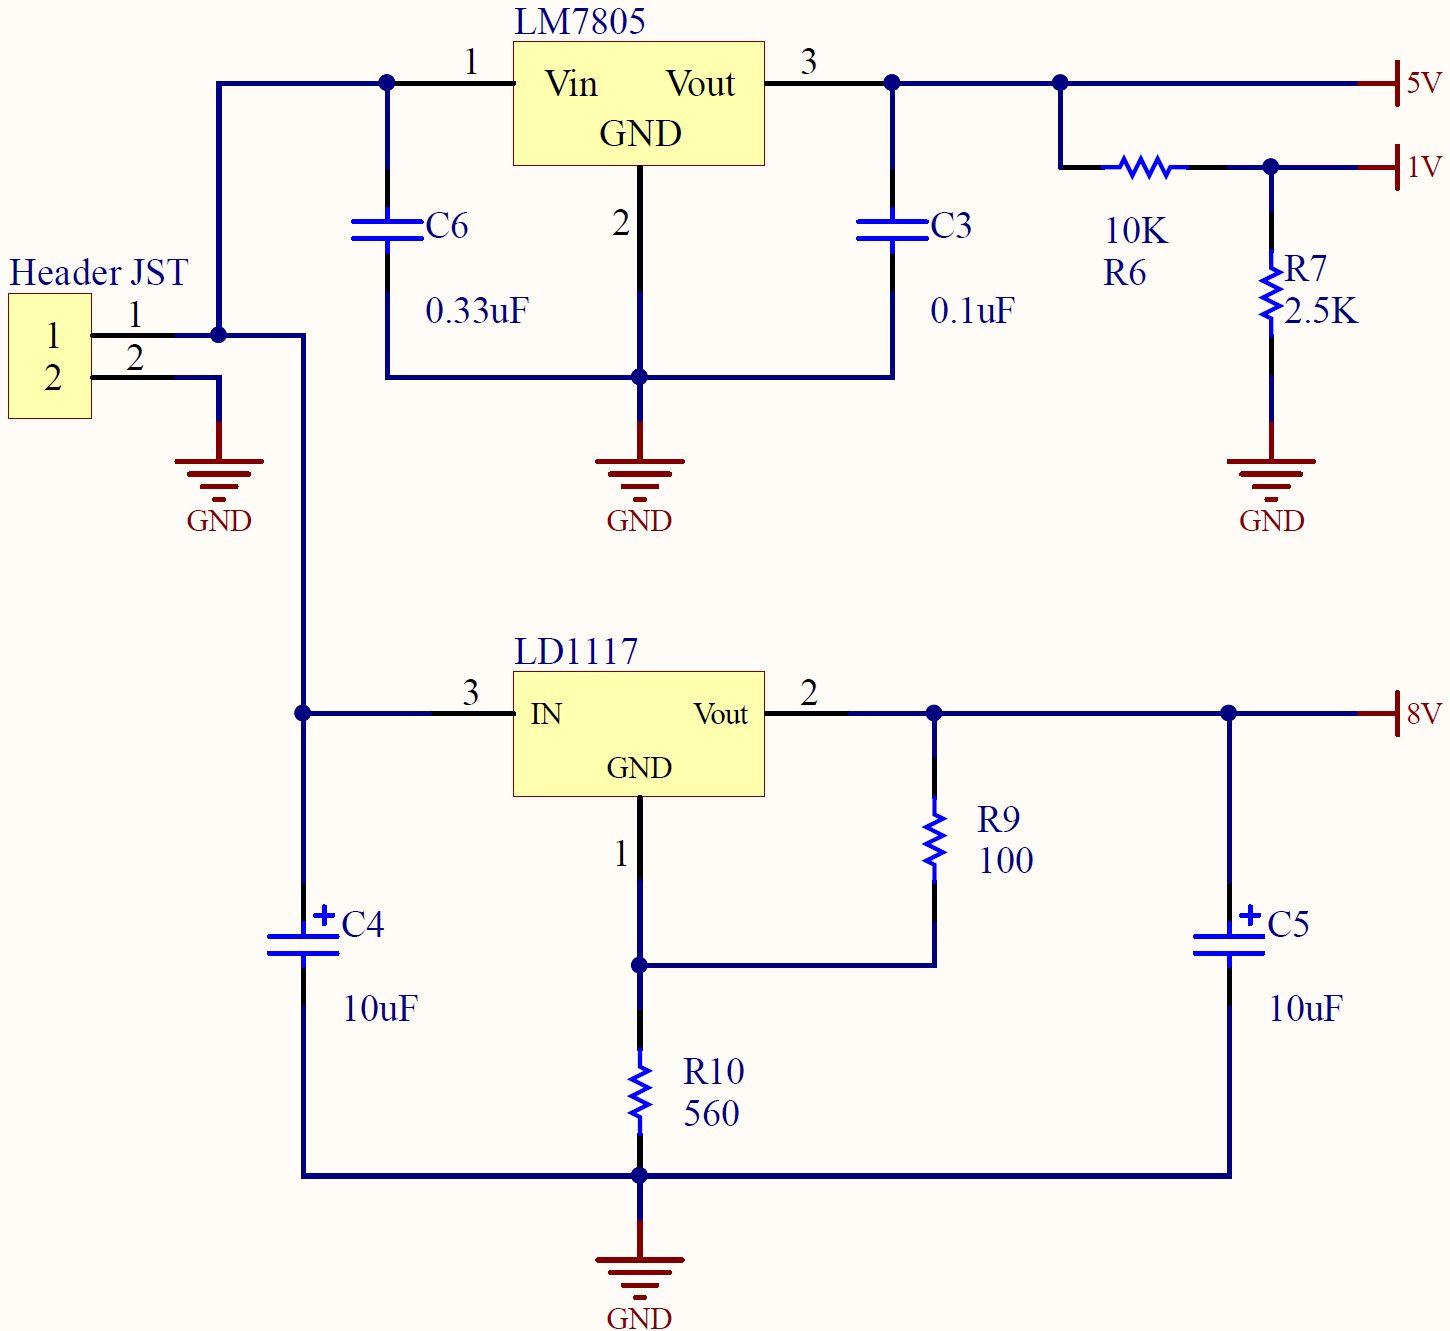
\includegraphics[width=0.6\textwidth]{./image/CircuitoFuente.png}
\caption{Etapa 1, Fuentes de 5V, 8V y Referencia de 1V.}
\label{fig:EtapaFuente}
\end{figure}

En la etapa (1) de alimentación de la tarjeta se usaron dos reguladores de voltaje para asegurar dos fuentes una de 5 Voltios y otra de 8 Voltios, y un voltaje de referencia como señal para la entrada al amplificador operacional de 1 Voltio. Para la fuente de 5 Voltios se utilizó un integrado de montaje superficial \href{https://www.sparkfun.com/datasheets/Components/LM7805.pdf}{LM7805}, este es utilizado para alimentar el microcontrolador \href{http://ww1.microchip.com/downloads/en/DeviceDoc/30487c.pdf}{PIC16F88}, el modulo \href{https://www.olimex.com/Products/Components/RF/BLUETOOTH-SERIAL-HC-06/resources/hc06.pdf}{Bluetooth HC-06}, darle Reset a la Tarjeta y derivar 1 Voltio para la referencia de los amplificadores operacionales por medio de un divisor de tensión. La regulación de 8 Voltios lograda con un integrado \href{https://cdn-shop.adafruit.com/product-files/2165/LD1117.pdf}{LD1117} es utilizada para la alimentación de dos amplificadores operacionales (\href{http://www.ti.com/lit/ds/symlink/lm158-n.pdf}{LM358} y \href{http://www.ti.com/lit/ds/symlink/lm124-n.pdf}{LM324}) cumpliendo así que este valor sea 2 Voltios mayor al máximo valor obtenido en la salida (OUT) de los amplificadores. El integrado \href{https://cdn-shop.adafruit.com/product-files/2165/LD1117.pdf}{LD1117} es un regulador variable y su ajuste viene definido por la siguiente ecuación:
\begin{center}
${{V}_{OUT}}={{V}_{REF}}(1+{{R}_{2}}/{{R}_{1}})$
\end{center}
Con base en el circuito que recomienda el fabricante (figura \ref{fig:circuitoejemplo}) y su ecuación podemos calcular el voltaje de salida de la siguiente manera:
\begin{figure}[H]
\centering
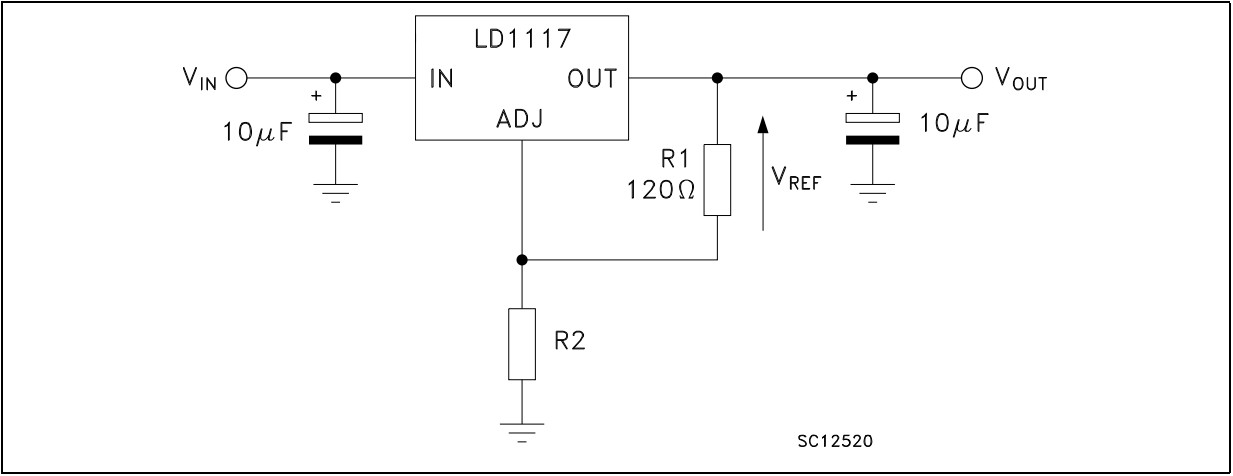
\includegraphics[width=0.9\textwidth]{./image/circuitoejemplo.png}
\caption{Aplicación de salida con voltaje ajustable. Fuente: \href{https://cdn-shop.adafruit.com/product-files/2165/LD1117.pdf}{LD1117}.}
\label{fig:circuitoejemplo}
\end{figure}
Dándole valores constantes a ${V}_{REF}=1.25V$, ${V}_{OUT}=8V$ y ${R}_{1}=100\Omega$ procedemos a despejar ${R}_{2}$:
\begin{center}
${R}_{2}=(({V}_{OUT}/{V}_{REF})-1)\times{R}_{1}$\\
${R}_{2}=((8V/1.25V)-1)\times100\Omega$\\
${R}_{2}=540\Omega$
\end{center}

\begin{figure}[H]
\centering
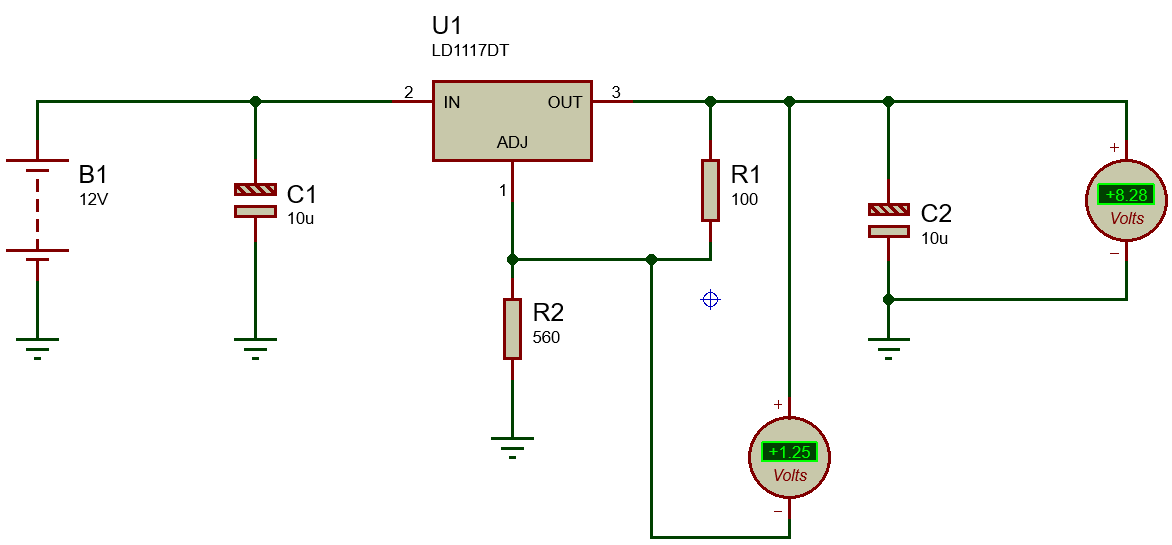
\includegraphics[width=0.9\textwidth]{./image/Simulacion_LD1117.png}
\caption{Simualción del circuito para el voltaje ajustable a 8V.}
\label{fig:SimulacionLD1117}
\end{figure}

Como buena practica se realizó la simulación en el software Proteus, el cual arrojó el resultado observado en la figura \ref{fig:SimulacionLD1117}.

En la etapa (2) (figura \ref{fig:EtapaAdquisicion}) encontramos la parte de adquisición, acondicionamiento y entrega de datos al microcontrolador, esta etapa esta compuesta por dos amplificadores operacionales un \href{http://www.ti.com/lit/ds/symlink/lm158-n.pdf}{LM358} el cual contiene dos amplificadores usados para los sensores 1 y 2 de la plantilla y un \href{http://www.ti.com/lit/ds/symlink/lm124-n.pdf}{LM324} que tiene los cuatro amplificadores usados para los sensores 3, 4 y 5. Estos amplificadores operacionales cumplen la función de proteger el circuito del microcontrolador de impedancias altas en las entradas del mismo.

\begin{figure}[H]
\centering
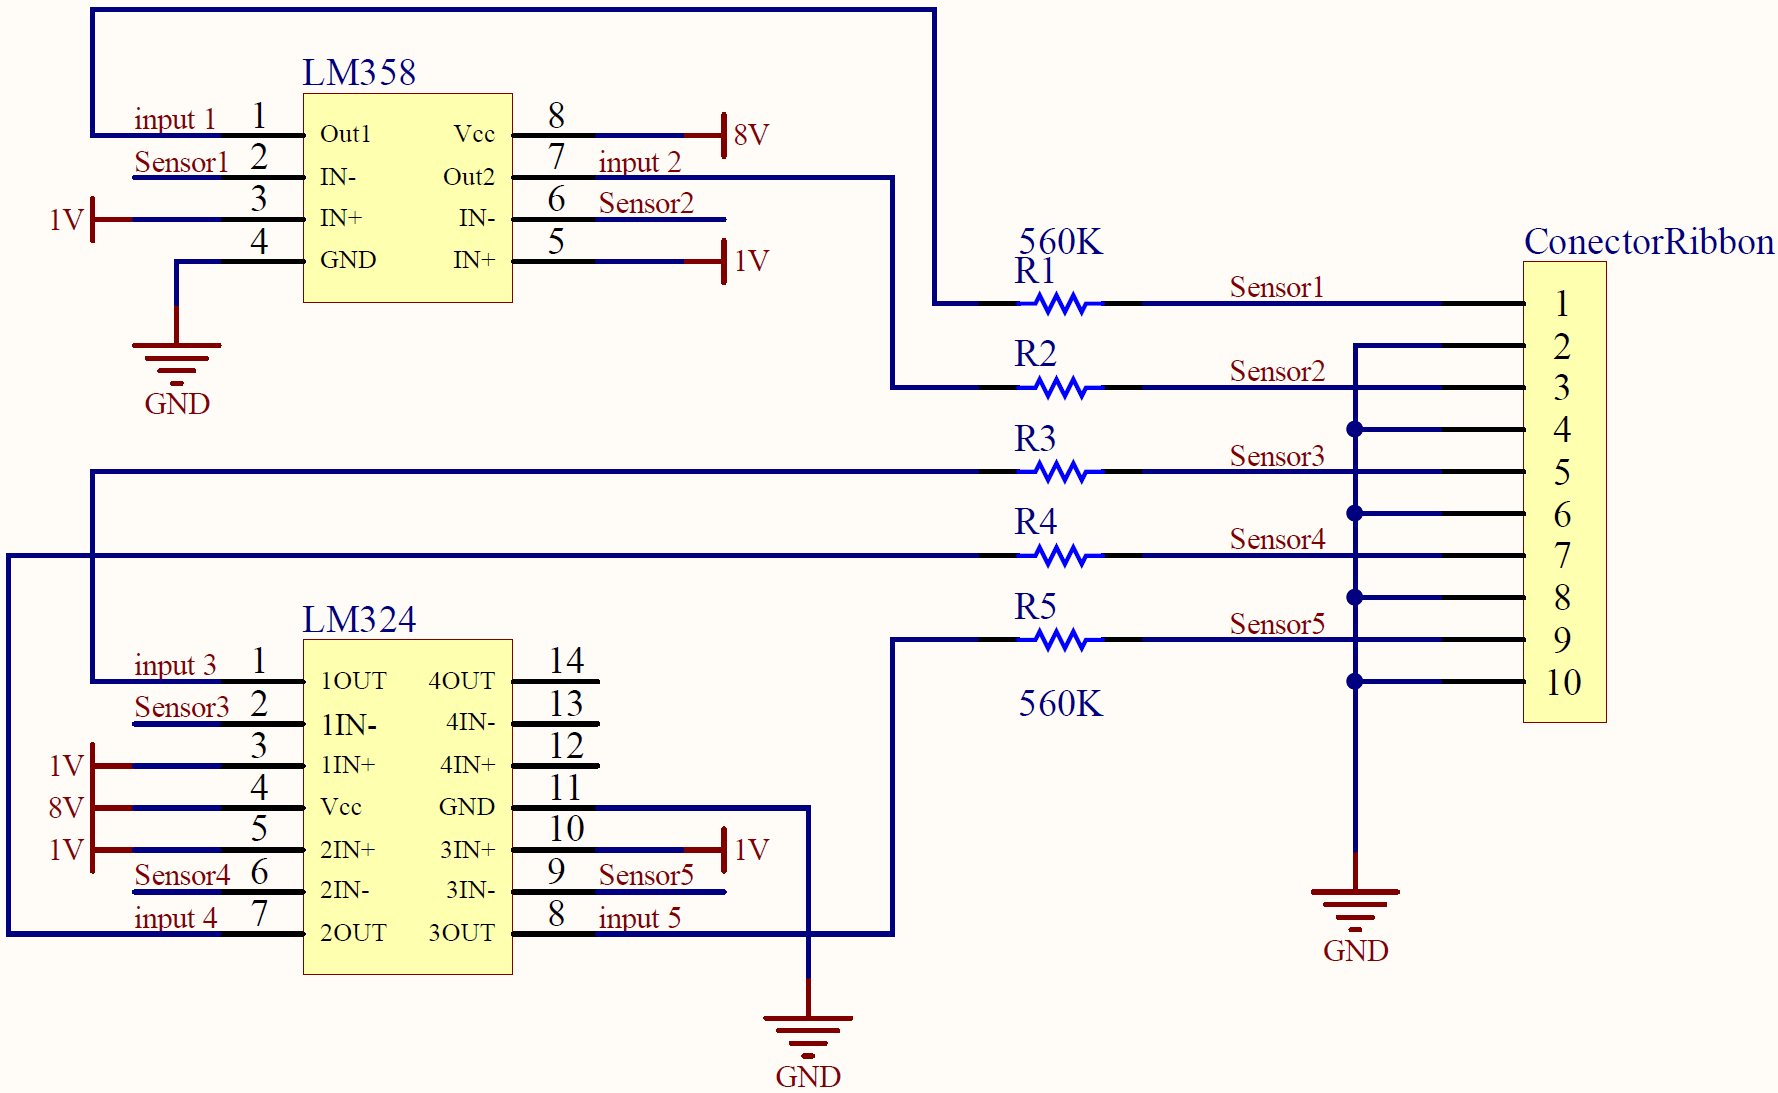
\includegraphics[width=0.7\textwidth]{./image/EtapaAdquisicionDatos.png}
\caption{Etapa 2, Etapa de Amplificadores Operacionales para la adquisición y acondicionamiento de los datos reflejados de cada Sensor.}
\label{fig:EtapaAdquisicion}
\end{figure}

\begin{figure}[H]
\centering
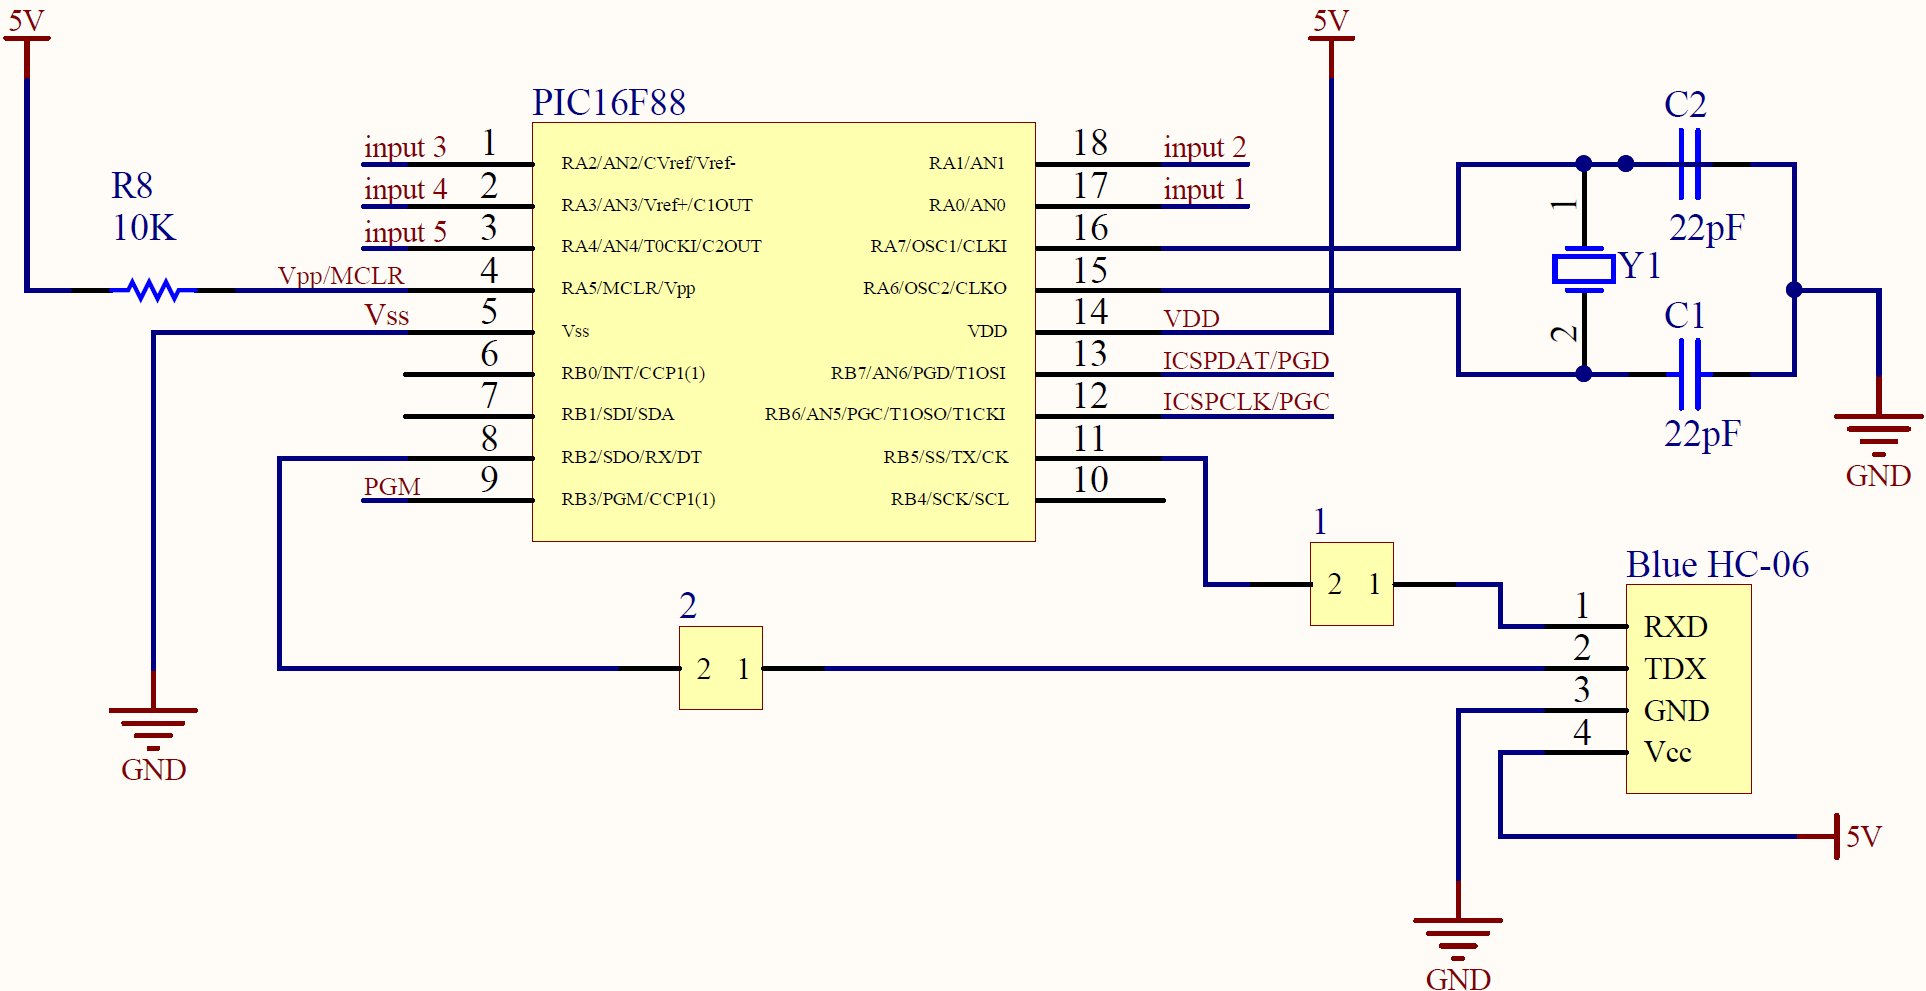
\includegraphics[width=0.7\textwidth]{./image/CircuitouControl.png}
\caption{Etapa 3, Etapa de procesamiento y envío mediante Bluetooth de los datos.}
\label{fig:EtapaProcesamiento}
\end{figure}

La etapa (3) esta compuesta por un microcontrolador de montaje superficial \href{http://ww1.microchip.com/downloads/en/DeviceDoc/30487c.pdf}{PIC16F88} el cual recibe los datos de los amplificadores operacionales y los procesa para posteriormente enviarlos por el puerto serie hacia el Bluetooth HC-06 y este último se encarga de hacer enlace con el computador con su antena a 2.4GHz.

\begin{figure}[H]
\centering
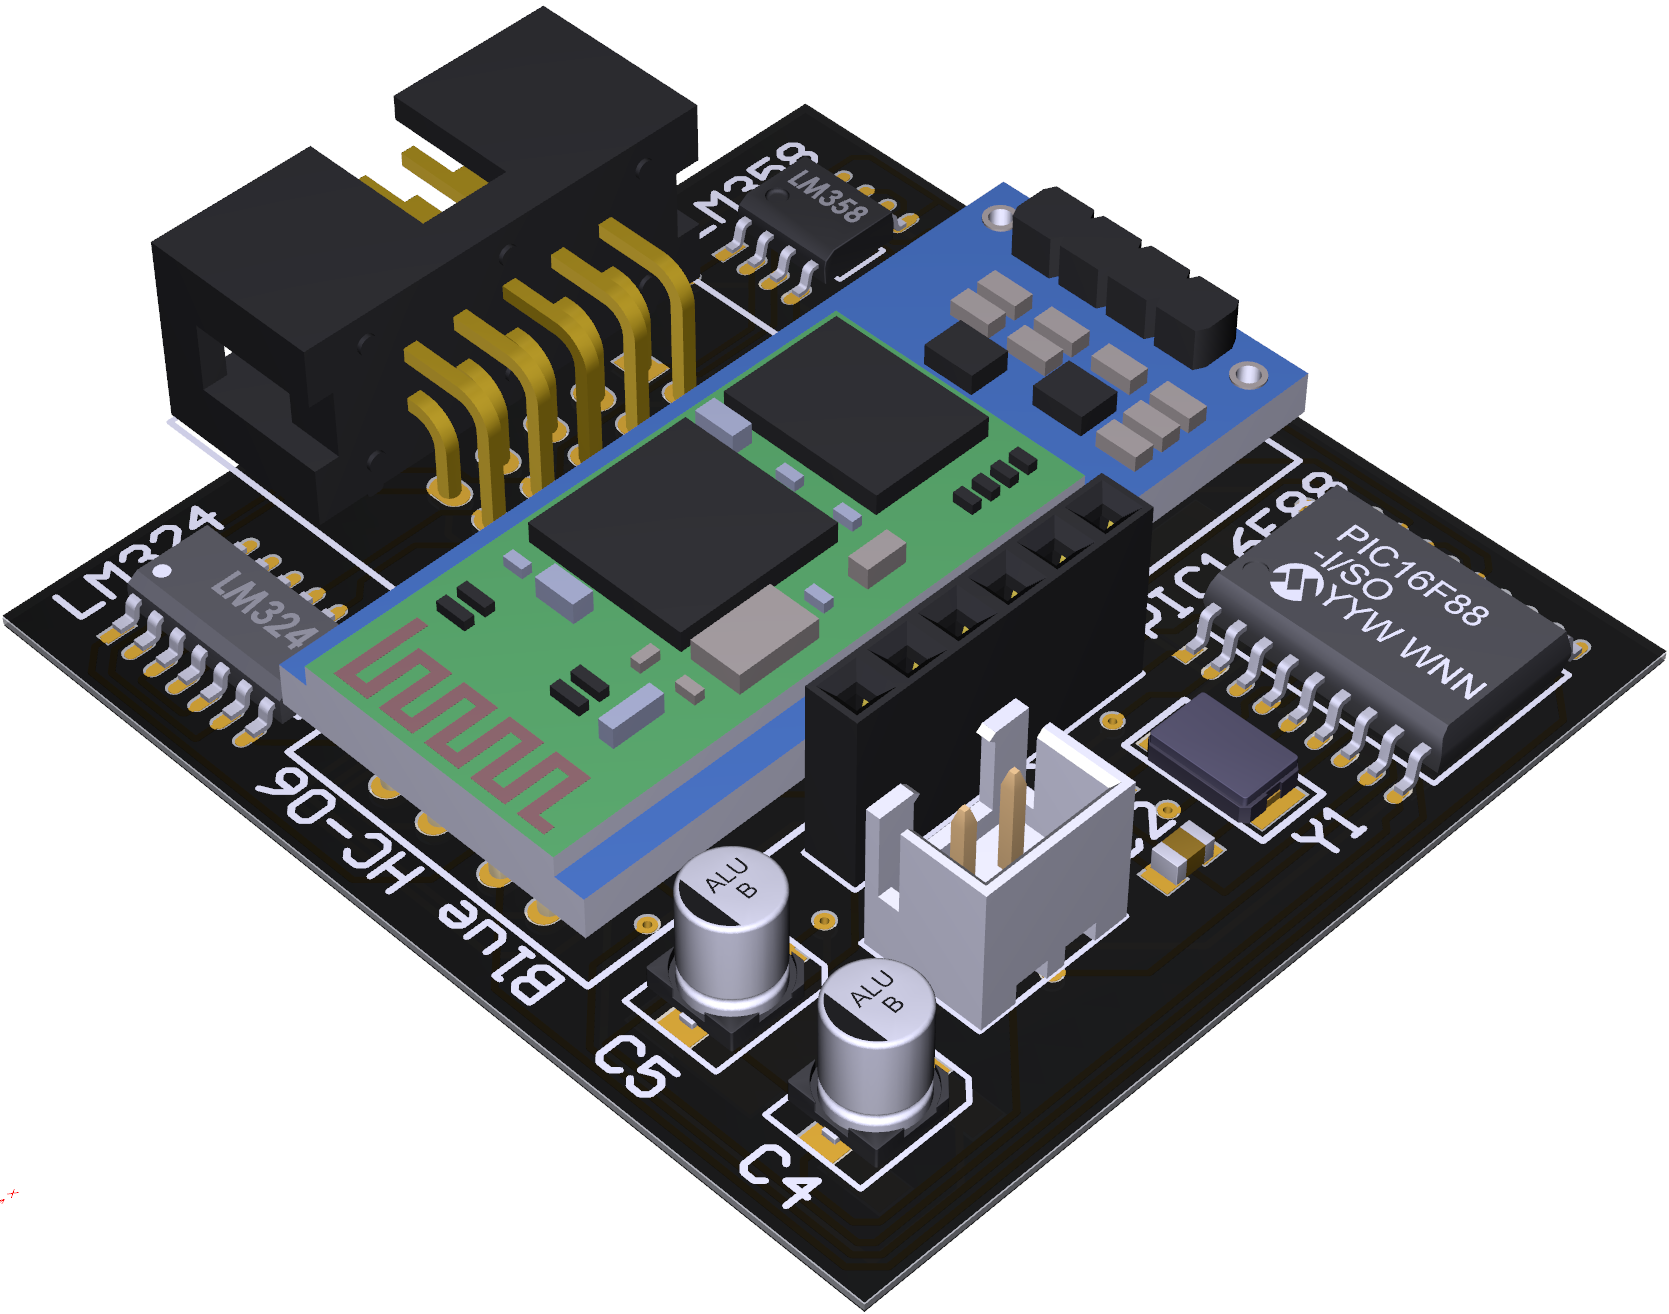
\includegraphics[width=0.7\textwidth]{./image/CircuitoSMD.png}
\caption{Tarjeta 3D de Adquisición, Procesamiento y envío de Datos.}
\label{fig:CircuitoSMD}
\end{figure}

\section{Calibración de Sensores}

En esta etapa se efectuaron pruebas de fuerza con 5 sensores de igual capacidad. Se realizaron pruebas con distintos valores de fuerza en los sensores y se obtuvieron mediciones similares entre sí, con lo cual se verificó que la calibración fue correcta. En la Fig. \ref{fig:Comportamiento} se puede observar los diferentes comportamientos para cada sensor de forma individual y con mas detalle se pueden ver estos valores en la Tabla \ref{Table:Valores}. Resulta importante aclarar que cada sensor arrojó valores que difieren un poco pero siguen un mismo patrón de forma lineal siendo su resistencia inversamente proporcional a la presión ejercida en cada sensor.

\begin{table}[H]
%\small
%\footnotesize
\scriptsize
%\tiny
\begin{center}
\begin{tabular}{| c | c | c | c | c | c |}
 \hline
\textbf{Sensor} & \textbf{Medida} & \textbf{Fuerza [KN]} & \textbf{Voltaje [V]} & \textbf{Voltaje min.} & \textbf{Voltaje max.} \\ 
 \hline
                    & 1 & 0,059 & 1,99 & 1,93 & 2,05 \\  
                    & 2 & 0,12 & 2,05 & 1,97 & 2,12 \\
                    & 3 & 0,168 & 2,33 & 2,28 & 2,37 \\
    1               & 4 & 0,205 & 2,62 & 2,57 & 2,68 \\
                    & 5 & 0,31 & 2,76 & 2,72 & 2,80 \\
                    & 6 & 0,432 & 3,75 & 3,73 & 3,77 \\
 \hline
                    & 7 & 0,06 & 2,10 & 2,04 & 2,16 \\
 					& 8 & 0,13 & 2,34 & 2,28 & 2,40 \\
    2               & 9 & 0,2 & 2,66 & 2,61 & 2,71 \\  
 					& 10 & 0,32 & 2,86 & 2,82 & 2,89 \\
 					& 11 & 0,42 & 3,02 & 2,99 & 3,06 \\
 \hline
					& 12 & 0,055 & 2,02 & 1,94 & 2,11 \\
					& 13 & 0,0115 & 2,11 & 2,05 & 2,18 \\
    3				& 14 & 0,21 & 2,39 & 2,34 & 2,45 \\
					& 15 & 0,3 & 2,55 & 2,45 & 2,65 \\
					& 16 & 0,43 & 2,86 & 2,82 & 2,91 \\
 \hline
					& 17 & 0,06 & 2,12 & 2,06 & 2,19 \\  
 					& 18 & 0,139 & 2,54 & 2,49 & 2,58 \\
	4				& 19 & 0,2 & 2,94 & 2,89 & 2,99 \\
					& 20 & 0,33 & 3,36 & 3,32 & 3,39 \\
					& 21 & 0,43 & 3,87 & 3,82 & 3,92 \\
 \hline
					& 22 & 0,055 & 1,96 & 1,83 & 2,08 \\
					& 23 & 0,13 & 2,05 & 1,93 & 2,17 \\
	5				& 24 & 0,215 & 2,34 & 2,29 & 2,38 \\
					& 25 & 0,315 & 2,61 & 2,58 & 2,64 \\
					& 26 & 0,435 & 3,41 & 3,36 & 3,45 \\
 \hline
\end{tabular}
\caption{Valores obtenidos en la caracterización de cada sensor.}
\label{Table:Valores}
\end{center}
\end{table}

\begin{figure}[H]
\centering
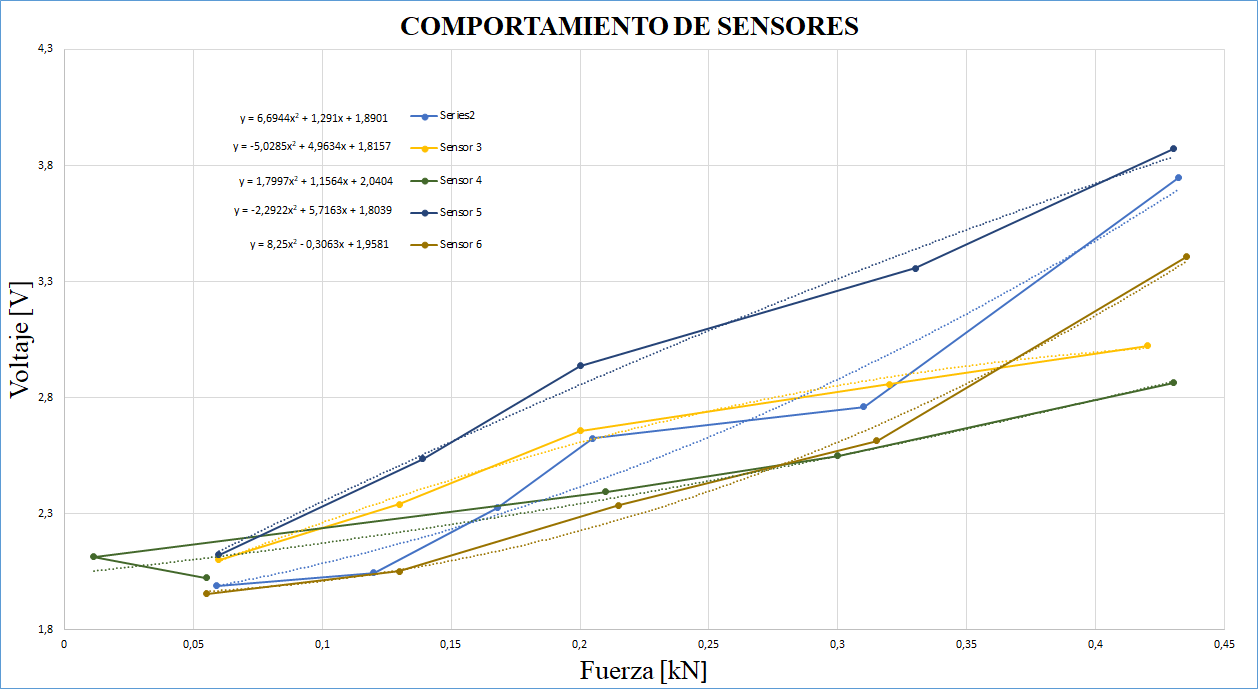
\includegraphics[width=1\textwidth]{./image/ComportamientoSensores.png}
\caption{Gráfica obtenida de la calibración de sensores.}
\label{fig:Comportamiento}
\end{figure}

\begin{figure}[H]
\centering
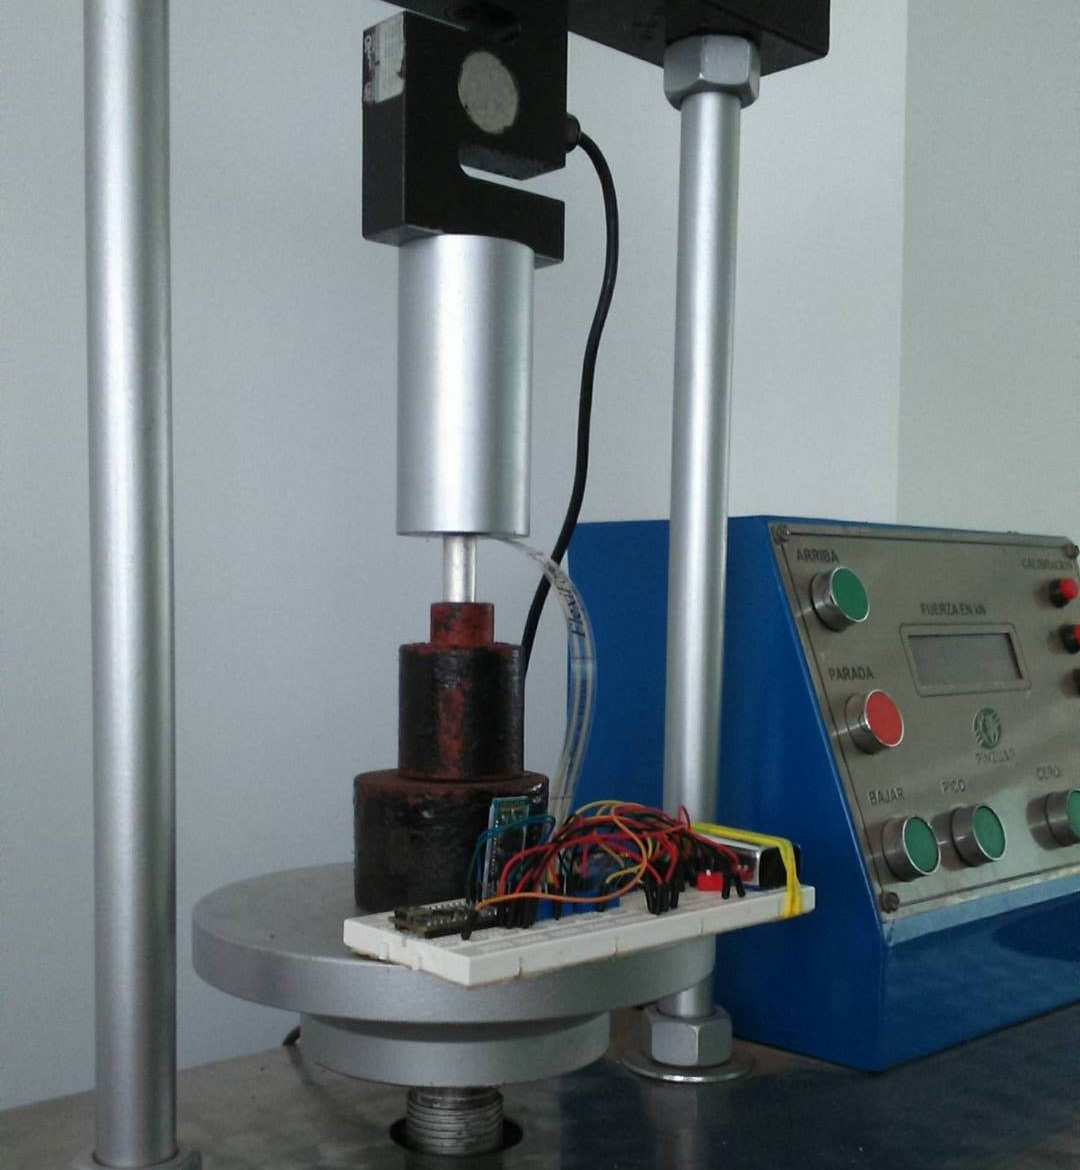
\includegraphics[width=0.5\textwidth]{./image/2.jpg}
\caption{Montaje para la calibración de sensores.}
\label{fig:Montaje}
\end{figure}

Para la calibración de estos sensores el montaje utilizado se puede visualizar en la Fig. \ref{fig:Montaje} donde se utilizó la maquina semiautomática digital para ensayos Marshall y CBR del laboratorio de suelos de la Universidad Tecnológica de Bolívar.

La Máquina Digital para Ensayos Marshall y CBR PS-25 esta diseñada para la exactitud, rapidez y registro confiable de los resultados adquiridos. Cuenta con un mecanismo de operación manual por medio de manivela para los ensayos de CBR (California Bearing Ratio: Ensayo de Relación de Soporte de California) mide la resistencia al esfuerzo cortante de un suelo en cemento, y operación eléctrica para el ensayo Marshall determina valores de estabilidad y deformabilidad de los pavimentos asfálticos; con medición digital de fuerza, desplazamiento (penetración, deformación o flujo) y velocidad de avance. Así mismo registra la deformación y la carga máxima (pico) en 12 puntos de deformación vs. fuerza en ensayo CBR, e incluye un seguro electro-mecánico que impide la operación eléctrica cuando está puesta la manivela (biela).

Especificaciones Técnicas:

\begin{itemize}
\item Rango de fuerza (Estabilidad): 0 a 50 kN compresión.
\item Clase de exactitud: 0,5 \% desde el 10 \% del rango.
\item Celdas de carga: 1 celda tipo “S” compresión | Rango: 0 a 50 kN.
\item Rango de desplazamiento (penetración, elongación y flujo): 50 mm.
\item Exactitud de la medición de desplazamiento: $0,1 \% \pm 0,05 mm$.
\item Velocidad de desplazamiento con operación eléctrica para ensayo Marshall $50,8 mm$.
\item Operación: 110 VAC (Opcional 220 VAC).
\item Dimensiones totales: $505 mm \times 775 mm \times 1 100 mm$.
\item Peso: 132 kg.
\end{itemize}


\section{Aplicación}

La aplicación debe cumplir ciertos criterios para su desarrollo entre ellos están: 

\begin{itemize}
\item El programa debe ser intuitivo
\item Gráfica en tiempo real
\item Debe ser visualizado en todo tipo de dispositivo conectado a Internet
\end{itemize}

Para lograr lo anteriormente mencionado se recurre a las herramientas de \href{https://nodejs.org/es/}{Node Js} entorno construido con el motor de JavaScript V8 de Chrome usando un módulo de operaciones E/S y orientado a eventos y ademas contiene el ecosistema mas grade de librerías de código abierto, \href{https://atom.io/}{Atom} editor de texto de fuente de codigo abierto, y librerías como Serialport que permitirá recibir e interpretar los datos recibidos por el puerto COM, y en este caso los recibidos vía Bluetooth, \href{http://expressjs.com/es/}{Express} es un framework diseñado para la construcción de aplicaciones web y \href{https://www.chartjs.org/}{Chart Js} herramienta que nos permite desarrollar y diseñar gráficas en javascript.\\

El editor de texto \href{https://atom.io/}{Atom} nos brinda una mejor organización de todo el proyecto determinando cada archivo con su extensión y además incluye un terminal donde se activa el servidor y se llaman todos los archivos que la app necesita ejecutar para su funcionamiento.\\

El resultado de esta app Web brinda una aplicación que se ejecuta desde el servidor mostrando una gráfica (fig. \ref{fig:insoleweb}) en tiempo real con series de cada sensor que varían en función del movimiento y/o fuerza ejercida sobre la plantilla. Estos datos pueden ser interpretados por el entrenador o deportista para su posterior análisis de la técnica del ejercicio.

\begin{figure}[H]
 \centering
  \subfloat[Atom editor de texto]{
   \label{fig:Atom}
    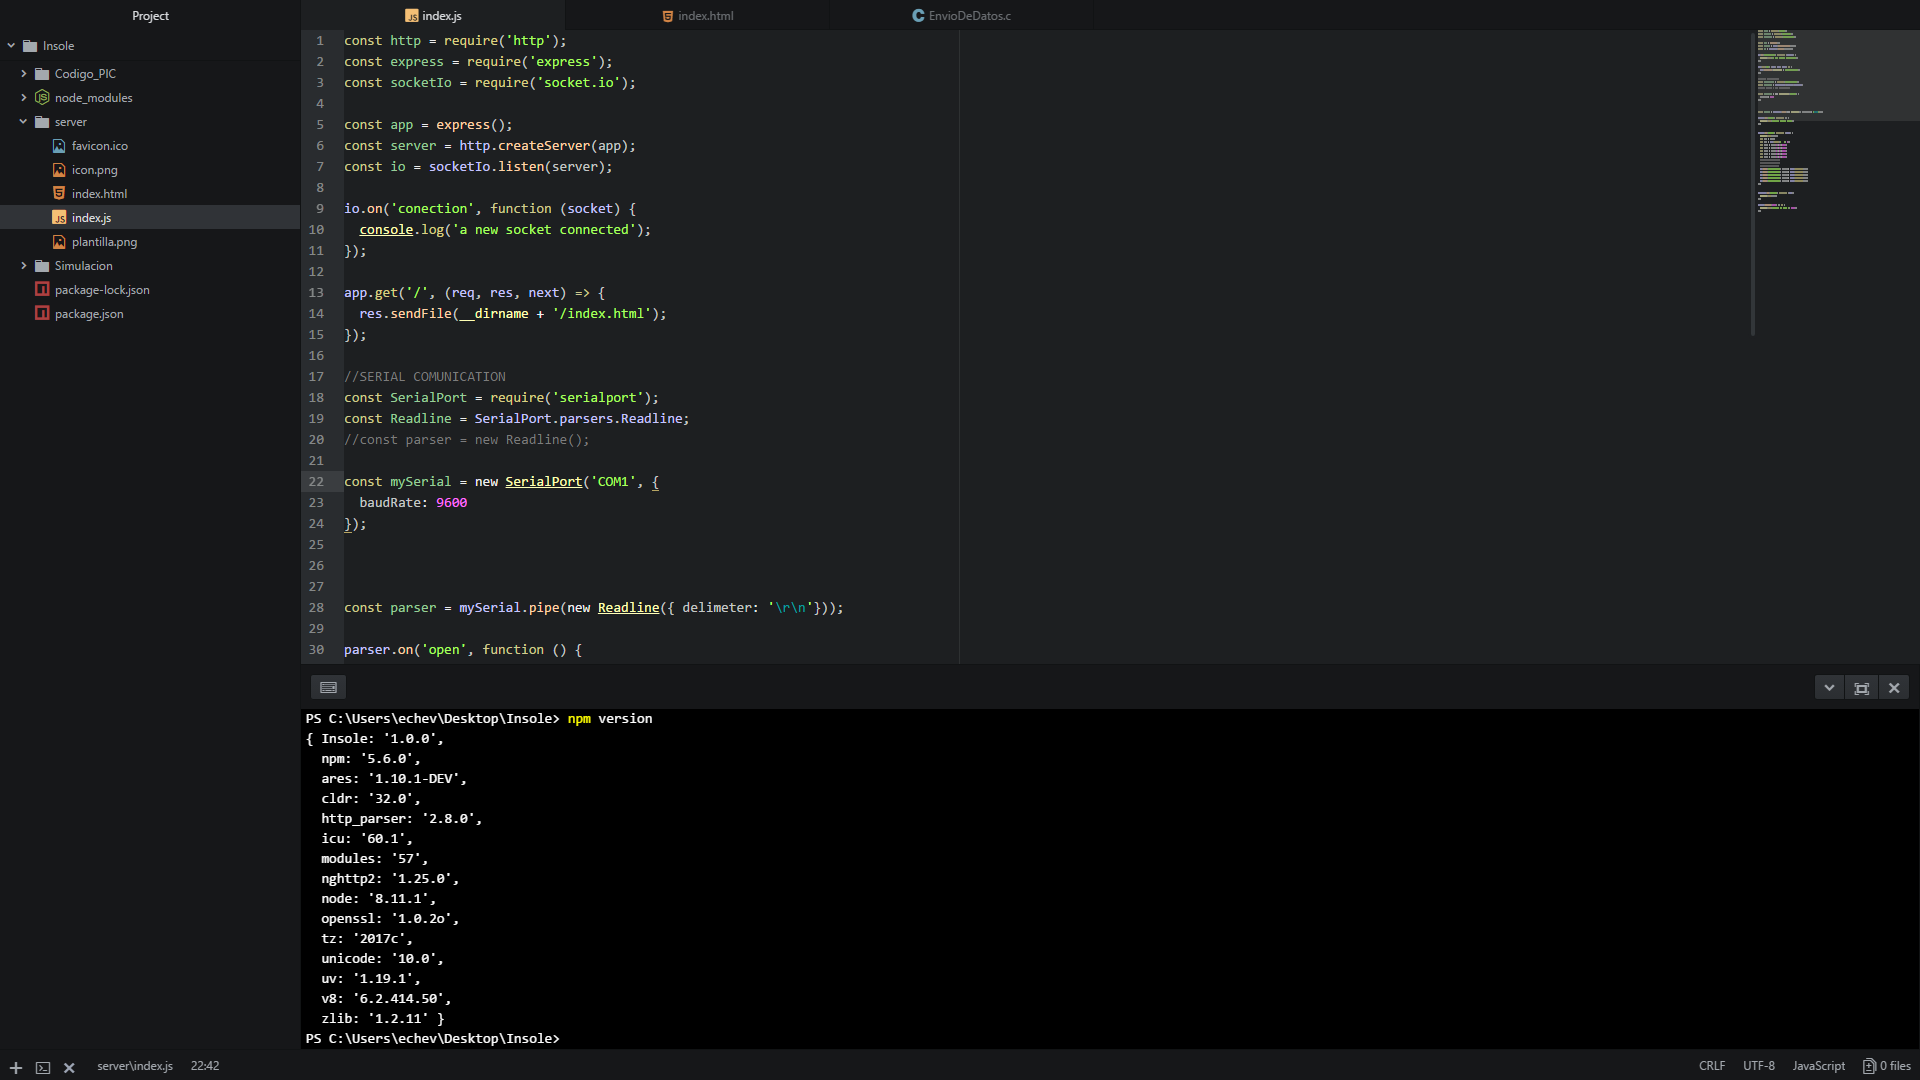
\includegraphics[width=1\textwidth]{./image/atom_image.png}}\\
    \subfloat[App Web desde cualquier navegador]{
   \label{fig:insoleweb}
    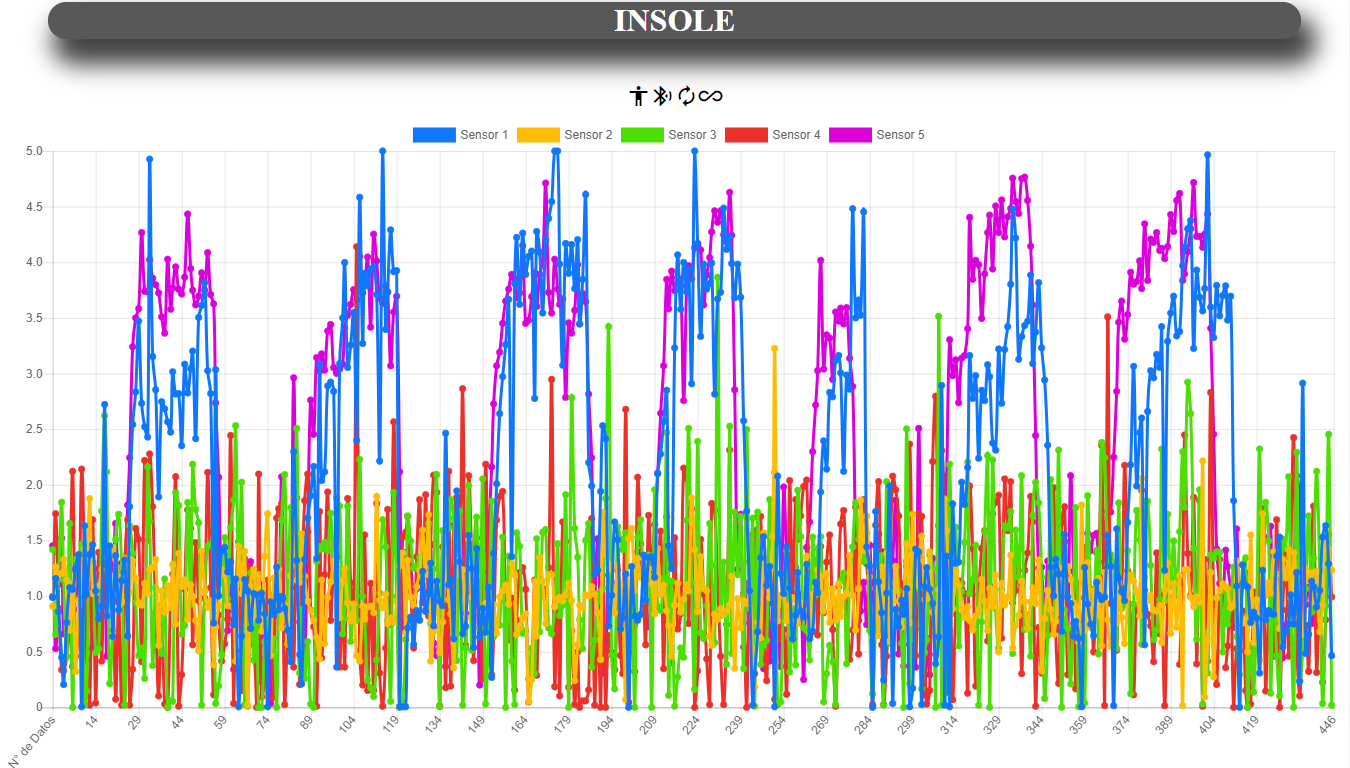
\includegraphics[width=1\textwidth]{./image/Insoleapp.png}}
 \caption{Software Utilizado para el desarrollo de la aplicación Web.}
 \label{fig:appWeb}
\end{figure}

